\documentclass{amsart}
\usepackage{amssymb,amsmath,amsthm,graphicx,hyperref}
\usepackage{textcomp}  

\usepackage{algorithm}
\usepackage{algpseudocode}

\newtheorem{theorem}{Theorem}
\newtheorem{proposition}{Proposition}
\newtheorem{lemma}{Lemma}
\theoremstyle{remark}
\newtheorem{remark}{Remark}

\title{Numerical methods precept 12}



\begin{document}

\maketitle

\subsection{Instructor} 
\begin{itemize}
\item Nicholas Marshall (\texttt{nicholas.marshall@princeton.edu})
\end{itemize}
\subsection{Teaching assistant}
\begin{itemize} 
\item Jihao Long (\texttt{jihaol@princeton.edu})
\end{itemize}


\subsection{Summary} 
Today we will consider explicit and implicit multi-step methods. In particular,
we will consider two explicit methods: Euler's method
$$
y_{j+1} = y_j + h f(x_j,y_j)
$$
and Adams-Bashforth
\begin{multline*}
y_{j+4} = y_{j+3} + \frac{h}{24} \left( 55 f(x_{j+3},y_{j+3}) 
\right. \\ \left.
-59
f(x_{j+2},y_{j+2}) + 37 f(x_{j+1},y_{j+1}) - 9 f(x_j,y_j)
\right),
\end{multline*}
and two implicit methods: implicit Euler's
$$
y_{j+1} = y_j + h f(x_{j+1},y_{j+1}),
$$
and Adams-Moulton method
\begin{multline*}
y_{j+3} = y_{j+2} + \frac{h}{24} \left(9 f(x_{j+3},y_{j+3}) 
 \right. \\ \left.
+19
f(x_{j+2},y_{j+2}) -5 f(x_{j+1},y_{j+1}) + f(x_j,y_j) \right).
\end{multline*}

\subsection*{Task 1} A large non-stiff system of equations. Suppose that $y \in
\mathbb{R}^n$ where $n = 500$. Consider the system of differential equations
$$
y' = \left(-I + \frac{\sin(x)}{2} A \right) y 
$$
where $A \in \mathbb{R}^{n \times n}$ is a symmetric matrix whose eigenvalues
are contained in the interval $[1/2,1]$ with the initial condition 
$$
y(0) = b,
$$
where $b \in \mathbb{R}^n$. The matrix $A$ and vector $b$ should be loaded from
the .mat file precept12.mat using load (In Python you can use scipy.io.loadmat).
Determine $y(1)$ using Euler's method to relative error less than $1e-4$.



\subsection*{Task 2} A small (1-dimensional) stiff system of equations. Suppose
that 
$$
y' = 100(\sin x - y), \qquad y(0) = 0.
$$
The exact solution is
$$
y(x) = \frac{\sin x - 0.01 \cos x + 0.01 e^{-100 x}}{1.0001}.
$$
Determine $y(1)$ using implicit Euler  with relative accuracy $1e-5$.

\subsection*{Task 3} Stiff differential equations often have the
property that solution curves will converge to a common curve regardless of the
initial condition. To visualize this, solve the stiff differential equation from
Task 2 for $100$ different values of $y(0)$ between $-1$ and $1$ use
$\text{plot}(x,y); \text{hold all}$ in a loop to plot all of these all on the
same plot. 


\subsection*{Task 4} Next we review integration on the torus.
Consider the function 
$$
f(x) = \exp(-4 x^2) +  \exp(-4 (|x|-\pi)^2)
$$
on the torus $[-\pi,\pi]$. Numerically, this function is smooth and periodic on
the torus since
$$
\exp(-4 \pi^2) = 7.1572e-18
$$
Here is a plot of the function
$$
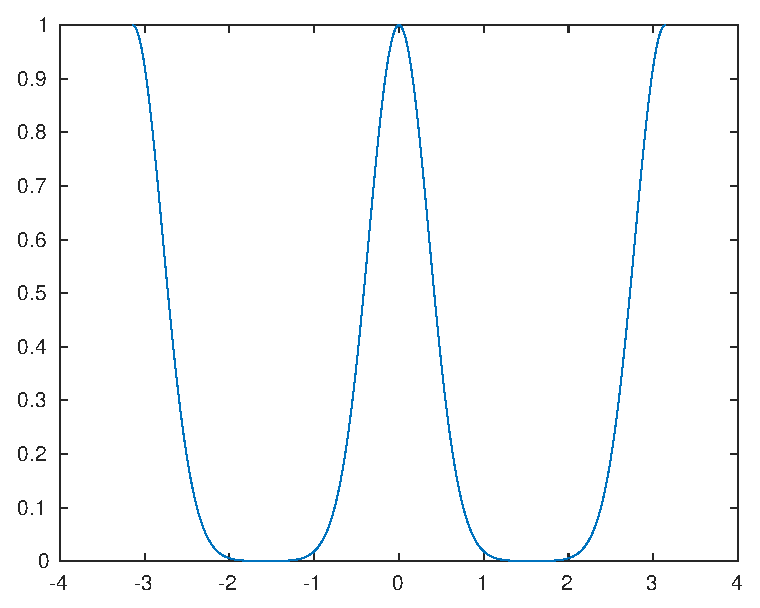
\includegraphics[width=.1\textwidth]{fig01.eps}
$$
Moreover, we have
$$
2 \int_{-\infty}^\infty e^{-4 x^2} dx = \sqrt{\pi}
$$
so the integral of this function on the torus should be $\sqrt{\pi}$ to machine
precision. By the Euler-Maclaurin formula we have that for any fixed $m$
$$
T(n) = \sqrt{\pi} + \mathcal{O}\left(\frac{1}{n^{2m}} \right),
$$
where $T(n)$ denotes trapezoid rule  with $n$ points (note that since the
function is periodic, trapezoid rule reduces to summing the function at equally
spaced points). That is, eventually
trapezoid rule will converge to the integral faster than $n^{-2m}$ for any $m$.
The issue is that the constant in the Big-O depends on $m$ so initially the
error rate might appear to be $n^{-2}$ until we ``overcome'' the constant.
To visualize this, run the code:
\begin{verbatim}
f = @(x) exp(-4*x.^2) + exp(-4*(abs(x)-pi).^2);
m = 200;
err = zeros(m,1);
for j = 1:m
    n = 2*j;
    h = 2*pi/n;
    x = -pi:h:pi-h;
    v = h*sum(f(x));
    err(j) = abs(v - sqrt(pi));
end

ms = 2*(1:m);
plot(log10(ms),log10(err)); hold all;
for j = 2:2:8
    ref = log10(ms.^-j) - log10(2^-j)+log10(err(1));
    plot(log10(ms),ref)
end
\end{verbatim}

\subsection*{Bonus Task} Use Adams-Moulton and Adams-Bashforth to solve Tasks
1 and 2 to relative accuracy 1e-12.



\end{document}
